\documentclass[11pt,a4paper]{article}
\usepackage[utf8]{inputenc}
\usepackage[T1]{fontenc}
\usepackage[french]{babel}
\usepackage[margin=1.8cm]{geometry}
\usepackage{graphicx}
\usepackage{hyperref}
\usepackage{enumitem}
\usepackage{titlesec}

\setlist{nosep,leftmargin=1.2em}
\titlespacing*{\section}{0pt}{0.4em}{0.2em}
\titleformat{\section}{\normalfont\bfseries\large}{\thesection}{0.5em}{}
\setlength{\parskip}{0.2em}
\setlength{\parindent}{0pt}

\title{\vspace{-1.5cm}Rapport individuel --- It\'eration 1}
\author{Alexis Briend (\texttt{abd7852}) --- Projet Long SHDL}
\date{13 avril 2026}

\begin{document}
\maketitle
\vspace{-2em}

\section*{Contexte}
Responsable de la \textbf{structure g\'en\'erale} de l'application et de l'\textbf{interpr\'etation du SHDL} (\textsc{Scrum-23}). Objectif sprint~1~: poser les fondations techniques (arborescence, gestion de d\'ependances, grammaire SHDL et parser vers un AST exploitable par les modules aval).

\section*{Activit\'es r\'ealis\'ees}
\begin{itemize}
  \item \textbf{Squelette JavaFX/Gradle} (\texttt{src/main/java/fr/n7/shdl/}, packages \texttt{model}/\texttt{view}/\texttt{controller}, \texttt{module-info}, \texttt{build.gradle}).
  \item \textbf{Grammaire SHDL LL(1)} (\texttt{parser/ll1/grammar/})~: r\`egles d\'eclaratives, calcul \textsc{First}/\textsc{Follow}, v\'erificateur de conflits LL(1).
  \item \textbf{AST immuable} (\texttt{parser/ll1/ast/})~: hi\'erarchie \texttt{Node $\to$ Expression}/\texttt{Statement}, champs \texttt{final}, \texttt{List.copyOf}, non-null garanti, Visitor typ\'e \texttt{<R>}.
  \item \textbf{Parseur \`a descente r\'ecursive} avec lookahead~2 sur les instances et messages d'erreur contextuels (code + position + attendu).
  \item \textbf{Documentation}~: spec \texttt{docs/specs/}, plan \texttt{docs/plans/}, bilan \texttt{docs/sprint1/}.
\end{itemize}

\section*{R\'esultats}
\begin{itemize}
  \item \textbf{107 tests JUnit verts} sur 23 classes (grammaire, tokens, AST, visiteur, invariants runtime, cas n\'egatifs, bout-en-bout \texttt{ET}/\texttt{BasculeD}/\texttt{FsmSync}/\texttt{DecBCD}).
  \item \textbf{39 fichiers Java} sous \texttt{parser/ll1/}. Une limite grammaticale connue (\texttt{TERM\_REST}, wildcard FSM~/~STAR de r\`egle voisine) est document\'ee et couverte par un test n\'egatif, report\'ee au sprint~2.
  \item Revue critique interne~: cinq d\'efauts d\'etect\'es (traversal incomplet du \texttt{DefaultVisitor}, champs redondants, invariants manquants), tous corrig\'es avant fin de sprint.
\end{itemize}

\begin{center}
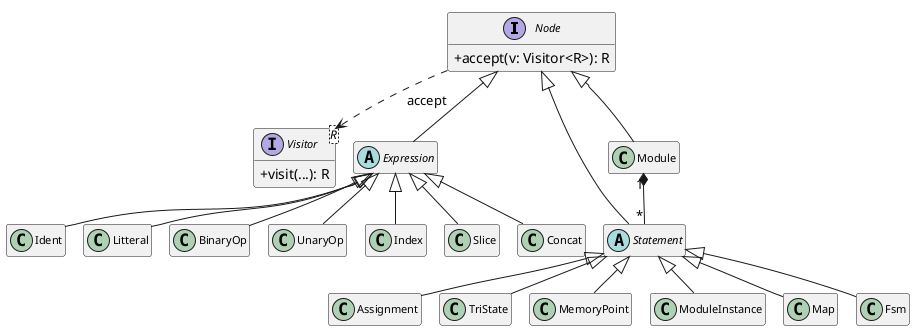
\includegraphics[width=0.75\textwidth]{ast-classes.png}\\
{\small Figure --- Diagramme de classes simplifi\'e de l'AST (source \texttt{ast-classes.puml}).}
\end{center}

\section*{Difficult\'es et r\'eussites}
Principale difficult\'e~: garantir que la grammaire reste \emph{r\'eellement} LL(1) apr\`es chaque ajout de r\`egle. Le v\'erificateur de conflits, \'ecrit \emph{avant} la grammaire, a d\'etect\'e plusieurs ambigu\"it\'es (instances de modules, FSM) sans aucune ex\'ecution du parser. R\'eussite~: l'immuabilit\'e stricte de l'AST, qui rend les passes aval (typage, automates) triviales \`a tester.

\section*{Manuel utilisateur}
Pr\'e-requis~: JDK~21+, JUnit~4 et Hamcrest dans \texttt{lib/}. Compilation et tests via \texttt{javac}/\texttt{org.junit.runner.JUnitCore} (commandes d\'etaill\'ees dans \texttt{docs/sprint1/}). Usage~: \texttt{new Parser(new Lexer(source)).parseFrom()} retourne l'AST racine \texttt{Module}, sur lequel un \texttt{Visitor<R>} ex\'ecute la passe aval choisie. Code sur \texttt{feature/skeleton-javafx}.

\end{document}
